\documentclass[11pt,a4paper]{article}

\usepackage{amsmath,amssymb,amsthm}
\usepackage{enumitem}
\usepackage{geometry}
\usepackage{hyperref}
\usepackage{xcolor}
\usepackage{float}
\usepackage{subcaption}
\usepackage{mdframed}
\usepackage{booktabs}
\usepackage{array}
\usepackage{tcolorbox}
\tcbuselibrary{skins, breakable}

\geometry{margin=1in}

% ── solution environment ─────────────────────────────────────────────────────
\newenvironment{solution}{%
    \begin{tcolorbox}[
        breakable,
        colback=green!4,
        colframe=green!50!black,
        fonttitle=\bfseries,
        title={Model Solution},
        left=6pt, right=6pt, top=4pt, bottom=4pt
    ]%
    }{%
    \end{tcolorbox}%
}


\newcommand{\todo}[0]{\textcolor{red}{TODO}}

\newcommand{\datei}[0]{\textcolor{blue}{Siehe auch abgegebenes R Skript}}

\usepackage{biblatex}
\addbibresource{seqan2.bib}

\title{Übung Postgenome Datensätze Teil 2 - Abgabe 1}
\author{Liliana Sanfilippo}
\date{}

\begin{document}

    \maketitle
    \datei
    \section{Berechnen sie zunächst zusätzliche Spalten}
    \subsection{Lesen sie die Daten mit einer tidyverse Funktion ein (bsp. read\_delim())}
    \begin{verbatim}
transkriptom <- read_delim("TrockenstressTag29.txt")

mapman <- read_delim("MapManTAIR10.txt")
descriptions <- read_delim("TAIR10_functional_descriptions_20150630.txt")
    \end{verbatim}
    \subsection{Berechnen sie Mittelwerte mit Hilfe von tidyverse Funktionen...}
    \begin{verbatim}
tpm_cols <- colnames(transkriptom)

print(tpm_cols)

transkriptom <- transkriptom %>%
  mutate(mean_D = rowMeans(across(matches("_D_r"))))
transkriptom <- transkriptom %>%
  mutate(mean_WW = rowMeans(across(matches("_WW_"))))
    \end{verbatim}

    \subsection{Erzeugen sie eine Funktion, die den log2-foldchange berechnet...}
    \begin{verbatim}
logtwofc <- function(x,y) {
   log2( (x+1) / (y+1) )
}
    \end{verbatim}

    \subsection{Nutzen sie die Funktion, um eine neue Spalte mit dem Namen d29Wvs29\_D\_log2FC
    zu erzeugen}
    \begin{verbatim}
transkriptom <- transkriptom %>%
  mutate(d29Wvs29_D_log2FC = logtwofc(mean_D, mean_WW))
    \end{verbatim}

    \section{Beantworten sie die folgenden Frage: Wie viele Transkripte haben in Kontrollbedingungen eine Abundanz grösser 1000, grösser 100, grösser 10?}
    \begin{verbatim}
# 10172
gr10 <- transkriptom |> filter(mean_WW > 10) |> tally()
# 1336
gr100 <- transkriptom |> filter(mean_WW > 100) |> tally()
#100
gr1000 <- transkriptom |> filter(mean_WW > 1000) |> tally()
    \end{verbatim}

    Größer als 10 haben 10172 Transkripte, größer als 100 haben 1336 und größer als 1000 haben 100.

    \section{Produzieren sie folgende Abbildungen}
    \subsection{Zusätzlich die Abb nur für die Kategorie Photosynthese}
    \begin{verbatim}
## Gennamen anpassen
transkriptom <- transkriptom %>%
  mutate(target_id_short = substr(target_id, 1, 9))
transkriptom <- transkriptom %>%
  mutate(neg_dek_p = -log10(d29Wvs29_D_q_value))
## Join
joined <- transkriptom %>% left_join(mapman, by = join_by("target_id_short" == "IDENTIFIER"))
## Nur PS
#ps <- joined |> filter(str_detect(across(NAME), pattern="PS."))
#ps <- joined |> filter(across(NAME, str_detect(pattern="PS.")))
ps <- joined |> filter(str_detect(substr(NAME, 1, 2), "PS"))
#ps <- transkriptom |> filter(starts_with("PS."))

j_cols <- colnames(joined)
    \end{verbatim}

    \subsection{Vulcano Plot...}

    \begin{verbatim}
zehn_top <- ps %>%
  slice_max(neg_dek_p, n=10)

volcano_plot <- ggplot(ps, aes(x = d29Wvs29_D_log2FC, y = neg_dek_p,
                                   color = ifelse(d29Wvs29_D_q_value < 0.01, "red", "black")
                                 )) +
  geom_point(size = 1) +
  labs(title = "Volcano Plot PS", x = "Log2FoldChange", y = "-log10(P-value)") +
  theme_minimal() +
  scale_color_manual(values = c("black", "red"),
                     labels = c("Nicht signifikant", "Signifikant"), name="Legende") +
  geom_text(data=zehn_top, aes(label=target_id), vjust= -0.5, show.legend = FALSE)

print(volcano_plot)

zehn_top <- joined %>%
  slice_max(neg_dek_p, n=10)

volcano_plot_all <- ggplot(joined, aes(x = d29Wvs29_D_log2FC, y = neg_dek_p,
                                   color = ifelse(d29Wvs29_D_q_value < 0.01, "red", "black")
)) +
  geom_point(size = 1) +
  labs(title = "Volcano Plot Alle", x = "Log2FoldChange", y = "-log10(P-value)") +
  theme_minimal() +
  scale_color_manual(values = c("black", "red"),
                     labels = c("Nicht signifikant", "Signifikant"), name="Legende") +
  geom_text(data=zehn_top, aes(label=target_id), vjust= -0.5, show.legend = FALSE)

print(volcano_plot_all)
    \end{verbatim}


    \begin{figure}[H]
        \centering
        
\includegraphics[width=0.6\linewidth]{pgd/volcanoPS.png}
        \caption{Vulcano Plot der Transkripte der Kategorie Photosynthese.}
    \end{figure}

    \begin{figure}[H]
        \centering
        
\includegraphics[width=0.6\linewidth]{pgd/volcanoAlle.png}
        \caption{Vulcano Plot aller Transkripte.}
    \end{figure}


    \subsection{Histogramm...}

    \begin{verbatim}

histo_data_all <- joined  %>% pivot_longer(
  cols = c(mean_D, mean_WW),
  names_to = "Bedingung",
  values_to = "Abundanzen"
)

histo_data_ps <- ps  %>% pivot_longer(
  cols = c(mean_D, mean_WW),
  names_to = "Bedingung",
  values_to = "Abundanzen"
)

###

histo_alle_einzeln <- ggplot(histo_data_all, aes(x = Abundanzen, fill= Bedingung)) +
  labs(title = "Histogramm Alle") +
  geom_histogram() +
  facet_wrap(~Bedingung) +
  scale_x_log10()

print(histo_alle_einzeln)

ggplot(histo_data_ps, aes(x = Abundanzen, fill= Bedingung)) +
  labs(title = "Histogramm PS") +
  geom_histogram() +
  facet_wrap(~Bedingung)
  scale_x_log10()

###

ggplot(histo_data_all, aes(x = Abundanzen, fill= Bedingung)) +
    labs(title = "Histogramm Alle") +
    geom_histogram(position="dodge") +
    scale_x_log10()

ggplot(histo_data_ps, aes(x = Abundanzen, fill= Bedingung)) +
    labs(title = "Histogramm PS") +
    geom_histogram(position="dodge") +
  scale_x_log10()
    \end{verbatim}

    \begin{figure}[H]
        \centering
        
\includegraphics[width=0.6\linewidth]{pgd/histoPS.png}
        \caption{Histogramm der Transkripte der Kategorie Photosynthese (zusammen).}
    \end{figure}

    \begin{figure}[H]
        \centering
        
\includegraphics[width=0.6\linewidth]{pgd/histoPSeinzeln.png}
        \caption{Histogramm der Transkripte der Kategorie Photosynthese (getrennt).}
    \end{figure}

    \begin{figure}[H]
        \centering
        
\includegraphics[width=0.6\linewidth]{pgd/histoAlle.png}
        \caption{Histogramm aller Transkripte (zusammen).}
    \end{figure}

    \begin{figure}[H]
        \centering
        
\includegraphics[width=0.6\linewidth]{pgd/histoAlleEinzeln.png}
        \caption{Histogramm aller Transkripte (einzeln).}
    \end{figure}

    \subsection{Boxplot...}
    \begin{verbatim}
ggplot(ps, aes(y = d29Wvs29_D_log2FC)) +
  labs(title = "Boxplot PS") +
  geom_boxplot()

ggplot(joined, aes(y = d29Wvs29_D_log2FC)) +
  labs(title = "Boxplot Alle") +
  geom_boxplot()
    \end{verbatim}

    \begin{figure}[H]
        \centering
        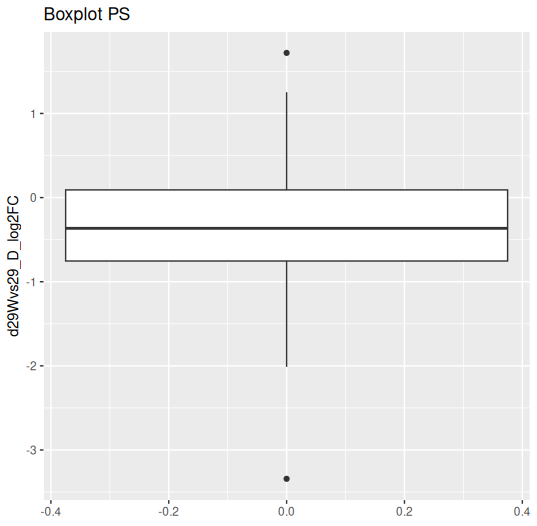
\includegraphics[width=0.6\linewidth]{boxplotPS}
        \caption{Boxplot der Transkripte der Kategorie Photosynthese.}
    \end{figure}

    \begin{figure}[H]
        \centering
        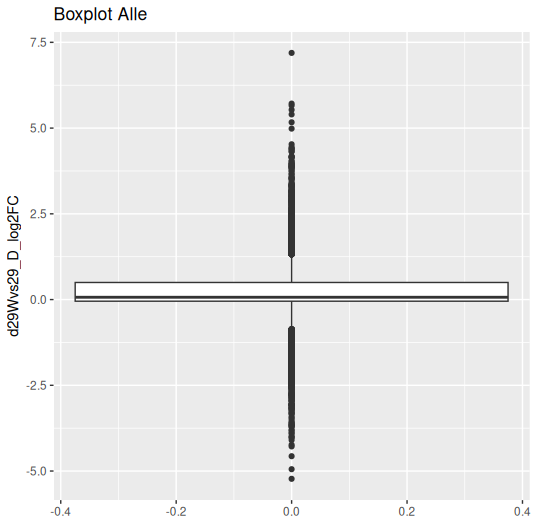
\includegraphics[width=0.6\linewidth]{boxplotAlle}
        \caption{Boxplot aller Transkripte.}
    \end{figure}

    \subsection{vergleichen sie mit der Abbildung aller Gene und
    kommentieren sie, ob und warum sie das Ergebnis so erwarten}
    Sehr grundlegend habe ich erwartet, dass die Graphen für die beiden Datensätze deutlich verschieden aussehen, da (nach visueller Überprüfung) wenig Datensätze der Kategorie Photosynthese in dem Gesamtdatensatz waren. Dies hat sich erfüllt.

    Außerdem würde ich erwarten, dass die Pflanzen unter Stress in den Überlebensmodus geht und deswegen die Photosyntheseaktivität heruntergeschraubt wird und es weniger Exprimierung von damit zusammenhängenden Genen gibt. In den Boxplots kann man gut sehen, dass die Verteilung der 2foldchange-Werte für den PS Datensatz im Gegensatz zum Gesamtdatensatz ins negative verschoben ist. Also bestätigt sich diese Vermutung.

    Im Valocano-Plot des PS-Datensatzen kann mman sehen, dass die meisten der Top-10-exprimierten Gene im linken/negativen (auf die x-Achse bezogenen) Bereich zu finden sind. Was auch darauf hinweist, dass diese unter Stress weniger exprimiert werden.
    Die Histrogramme sind weniger stark aussagekräftig, man sieht jedoch auch in Abb. 3, dass unter Trockenstress die meisten Abundanzen heruntergehen und ein paar sogar wegfallen.
\end{document}